\begin{figure}[H]
    \centering

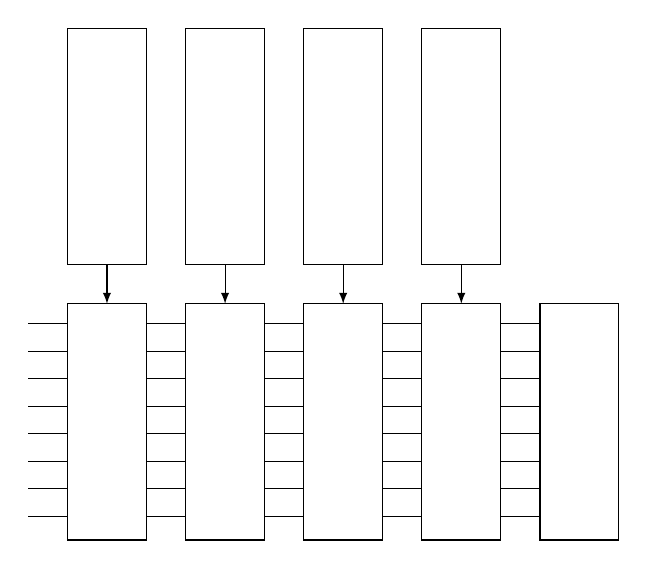
\begin{tikzpicture}[scale=.5]

\draw  (1,-15) rectangle (3,-21);
\draw
(3,-15.5)   to (4,-15.5)
(3,-16.2) to (4,-16.2)
(3,-16.9)  to (4,-16.9)
(3,-17.6) to (4,-17.6)
(3,-18.3) to (4,-18.3)
(3,-19) to (4,-19)
(3,-19.7) to (4,-19.7)
(3,-20.4) to (4,-20.4);

\draw  (4,-15) rectangle (6,-21);
\draw
(6,-15.5)   to (7,-15.5)
(6,-16.2) to (7,-16.2)
(6,-16.9)  to (7,-16.9)
(6,-17.6) to (7,-17.6)
(6,-18.3) to (7,-18.3)
(6,-19) to (7,-19)
(6,-19.7) to (7,-19.7)
(6,-20.4) to (7,-20.4);

\draw  (7,-15) rectangle (9,-21);
\draw
(9,-15.5)   to (10,-15.5)
(9,-16.2) to (10,-16.2)
(9,-16.9)  to (10,-16.9)
(9,-17.6) to (10,-17.6)
(9,-18.3) to (10,-18.3)
(9,-19) to (10,-19)
(9,-19.7) to (10,-19.7)
(9,-20.4) to (10,-20.4);

\draw  (10,-15) rectangle (12,-21);
\draw
(0,-15.5)   to (1,-15.5)
(0,-16.2) to (1,-16.2)
(0,-16.9)  to (1,-16.9)
(0,-17.6) to (1,-17.6)
(0,-18.3) to (1,-18.3)
(0,-19) to (1,-19)
(0,-19.7) to (1,-19.7)
(0,-20.4) to (1,-20.4);

\draw  (13,-15) rectangle (15,-21);
\draw
(12,-15.5)   to (13,-15.5)
(12,-16.2) to (13,-16.2)
(12,-16.9)  to (13,-16.9)
(12,-17.6) to (13,-17.6)
(12,-18.3) to (13,-18.3)
(12,-19) to (13,-19)
(12,-19.7) to (13,-19.7)
(12,-20.4) to (13,-20.4);

\draw  (1,-14) rectangle (3,-8);
\draw  (4,-14) rectangle (6,-8);
\draw  (7,-14) rectangle (9,-8);
\draw  (10,-14) rectangle (12,-8);

\draw [>=latex,->](2,-14) to (2,-15);
\draw [>=latex,->](5,-14) to (5,-15);
\draw [>=latex,->](8,-14) to (8,-15);
\draw [>=latex,->](11,-14) to (11,-15);

\end{tikzpicture}
    \caption{Method of transporting data from TDCs to the FPGA using a one bit serial shift register without shadowlatches}
    \label{tkz:serial_no_shadow}
\end{figure}
